% This is the Reed College LaTeX thesis template. Most of the work
% for the document class was done by Sam Noble (SN), as well as this
% template. Later comments etc. by Ben Salzberg (BTS). Additional
% restructuring and APA support by Jess Youngberg (JY).
% Your comments and suggestions are more than welcome; please email
% them to cus@reed.edu
%
% See http://web.reed.edu/cis/help/latex.html for help. There are a
% great bunch of help pages there, with notes on
% getting started, bibtex, etc. Go there and read it if you're not
% already familiar with LaTeX.
%
% Any line that starts with a percent symbol is a comment.
% They won't show up in the document, and are useful for notes
% to yourself and explaining commands.
% Commenting also removes a line from the document;
% very handy for troubleshooting problems. -BTS

% As far as I know, this follows the requirements laid out in
% the 2002-2003 Senior Handbook. Ask a librarian to check the
% document before binding. -SN

%%
%% Preamble
%%
% \documentclass{<something>} must begin each LaTeX document
\documentclass[12pt,twoside]{reedthesis}
% Packages are extensions to the basic LaTeX functions. Whatever you
% want to typeset, there is probably a package out there for it.
% Chemistry (chemtex), screenplays, you name it.
% Check out CTAN to see: http://www.ctan.org/
%%
\usepackage{graphicx,latexsym}
\usepackage{amsmath}
\usepackage{amssymb,amsthm}
\usepackage{longtable,booktabs,setspace}
\usepackage{chemarr} %% Useful for one reaction arrow, useless if you're not a chem major
\usepackage[hyphens]{url}
% Added by CII
\usepackage{hyperref}
\usepackage{lmodern}
\usepackage{float}
\floatplacement{figure}{H}
% End of CII addition
\usepackage{rotating}

% Next line commented out by CII
%%% \usepackage{natbib}
% Comment out the natbib line above and uncomment the following two lines to use the new
% biblatex-chicago style, for Chicago A. Also make some changes at the end where the
% bibliography is included.
%\usepackage{biblatex-chicago}
%\bibliography{thesis}


% Added by CII (Thanks, Hadley!)
% Use ref for internal links
\renewcommand{\hyperref}[2][???]{\autoref{#1}}
\def\chapterautorefname{Chapter}
\def\sectionautorefname{Section}
\def\subsectionautorefname{Subsection}
% End of CII addition

% Added by CII
\usepackage{caption}
\captionsetup{width=5in}
% End of CII addition

% \usepackage{times} % other fonts are available like times, bookman, charter, palatino

% Syntax highlighting #22
  \usepackage{color}
  \usepackage{fancyvrb}
  \newcommand{\VerbBar}{|}
  \newcommand{\VERB}{\Verb[commandchars=\\\{\}]}
  \DefineVerbatimEnvironment{Highlighting}{Verbatim}{commandchars=\\\{\}}
  % Add ',fontsize=\small' for more characters per line
  \usepackage{framed}
  \definecolor{shadecolor}{RGB}{248,248,248}
  \newenvironment{Shaded}{\begin{snugshade}}{\end{snugshade}}
  \newcommand{\KeywordTok}[1]{\textcolor[rgb]{0.13,0.29,0.53}{\textbf{#1}}}
  \newcommand{\DataTypeTok}[1]{\textcolor[rgb]{0.13,0.29,0.53}{#1}}
  \newcommand{\DecValTok}[1]{\textcolor[rgb]{0.00,0.00,0.81}{#1}}
  \newcommand{\BaseNTok}[1]{\textcolor[rgb]{0.00,0.00,0.81}{#1}}
  \newcommand{\FloatTok}[1]{\textcolor[rgb]{0.00,0.00,0.81}{#1}}
  \newcommand{\ConstantTok}[1]{\textcolor[rgb]{0.00,0.00,0.00}{#1}}
  \newcommand{\CharTok}[1]{\textcolor[rgb]{0.31,0.60,0.02}{#1}}
  \newcommand{\SpecialCharTok}[1]{\textcolor[rgb]{0.00,0.00,0.00}{#1}}
  \newcommand{\StringTok}[1]{\textcolor[rgb]{0.31,0.60,0.02}{#1}}
  \newcommand{\VerbatimStringTok}[1]{\textcolor[rgb]{0.31,0.60,0.02}{#1}}
  \newcommand{\SpecialStringTok}[1]{\textcolor[rgb]{0.31,0.60,0.02}{#1}}
  \newcommand{\ImportTok}[1]{#1}
  \newcommand{\CommentTok}[1]{\textcolor[rgb]{0.56,0.35,0.01}{\textit{#1}}}
  \newcommand{\DocumentationTok}[1]{\textcolor[rgb]{0.56,0.35,0.01}{\textbf{\textit{#1}}}}
  \newcommand{\AnnotationTok}[1]{\textcolor[rgb]{0.56,0.35,0.01}{\textbf{\textit{#1}}}}
  \newcommand{\CommentVarTok}[1]{\textcolor[rgb]{0.56,0.35,0.01}{\textbf{\textit{#1}}}}
  \newcommand{\OtherTok}[1]{\textcolor[rgb]{0.56,0.35,0.01}{#1}}
  \newcommand{\FunctionTok}[1]{\textcolor[rgb]{0.00,0.00,0.00}{#1}}
  \newcommand{\VariableTok}[1]{\textcolor[rgb]{0.00,0.00,0.00}{#1}}
  \newcommand{\ControlFlowTok}[1]{\textcolor[rgb]{0.13,0.29,0.53}{\textbf{#1}}}
  \newcommand{\OperatorTok}[1]{\textcolor[rgb]{0.81,0.36,0.00}{\textbf{#1}}}
  \newcommand{\BuiltInTok}[1]{#1}
  \newcommand{\ExtensionTok}[1]{#1}
  \newcommand{\PreprocessorTok}[1]{\textcolor[rgb]{0.56,0.35,0.01}{\textit{#1}}}
  \newcommand{\AttributeTok}[1]{\textcolor[rgb]{0.77,0.63,0.00}{#1}}
  \newcommand{\RegionMarkerTok}[1]{#1}
  \newcommand{\InformationTok}[1]{\textcolor[rgb]{0.56,0.35,0.01}{\textbf{\textit{#1}}}}
  \newcommand{\WarningTok}[1]{\textcolor[rgb]{0.56,0.35,0.01}{\textbf{\textit{#1}}}}
  \newcommand{\AlertTok}[1]{\textcolor[rgb]{0.94,0.16,0.16}{#1}}
  \newcommand{\ErrorTok}[1]{\textcolor[rgb]{0.64,0.00,0.00}{\textbf{#1}}}
  \newcommand{\NormalTok}[1]{#1}

% To pass between YAML and LaTeX the dollar signs are added by CII
\title{Mean Estimation via Neural Network Methods in Complex Survey Imputation}
\author{Alexander Michael Moore}
% The month and year that you submit your FINAL draft TO THE LIBRARY (May or December)
\date{May 2019}
\division{Mathematics and Statistics}
\advisor{Kelly McConville}
\institution{Reed College}
\degree{Bachelor of Arts}
%If you have two advisors for some reason, you can use the following
% Uncommented out by CII
% End of CII addition

%%% Remember to use the correct department!
\department{Mathematics}
% if you're writing a thesis in an interdisciplinary major,
% uncomment the line below and change the text as appropriate.
% check the Senior Handbook if unsure.
%\thedivisionof{The Established Interdisciplinary Committee for}
% if you want the approval page to say "Approved for the Committee",
% uncomment the next line
%\approvedforthe{Committee}

% Added by CII
%%% Copied from knitr
%% maxwidth is the original width if it's less than linewidth
%% otherwise use linewidth (to make sure the graphics do not exceed the margin)
\makeatletter
\def\maxwidth{ %
  \ifdim\Gin@nat@width>\linewidth
    \linewidth
  \else
    \Gin@nat@width
  \fi
}
\makeatother

\renewcommand{\contentsname}{Table of Contents}
% End of CII addition

\setlength{\parskip}{0pt}

% Added by CII

\providecommand{\tightlist}{%
  \setlength{\itemsep}{0pt}\setlength{\parskip}{0pt}}

\Acknowledgements{
I want to thank a few people.
}

\Dedication{
You can have a dedication here if you wish.
}

\Preface{
This is an example of a thesis setup to use the reed thesis document
class (for LaTeX) and the R bookdown package, in general.
}

\Abstract{
Abstract last. 100-500 words. Abstract should be able to stand alone:
results and approach blatantly and simply stated. Want to sell paper at
a glimpse
\begin{itemize}
\tightlist
\item
  main objectiuve and rationale of project
\item
  outline of methods used
\item
  results of the project
\item
  conclusions about the implications of the project
\end{itemize}
Missing data is problematic and pervasive in real surveys. Complex
survey imputation aims to replace missing data with approximations.
Modified neural networks (weighted loss, weighted resample,
\(\pi\)-feature, derived parameter) are compared to weighted linear
regression for mean estimation in artificial and real data using Monte
Carlo simulation on imputation of manually-induced missing data. The
methods' population mean estimates are compared to the known true mean
in both experiments. The results show the effectiveness of the neural
network family in low-noise nonlinear generative functions, and XXXXX in
Bureau of Labour Statistics Consumer Expenditure Survey data. Keras and
tensorFlow are utilized for neural network models.
}

% End of CII addition
%%
%% End Preamble
%%
%
\begin{document}

% Everything below added by CII
  \maketitle

\frontmatter % this stuff will be roman-numbered
\pagestyle{empty} % this removes page numbers from the frontmatter
  \begin{acknowledgements}
    I want to thank a few people.
  \end{acknowledgements}
  \begin{preface}
    This is an example of a thesis setup to use the reed thesis document
    class (for LaTeX) and the R bookdown package, in general.
  \end{preface}
  \hypersetup{linkcolor=black}
  \setcounter{tocdepth}{2}
  \tableofcontents

  \listoftables

  \listoffigures
  \begin{abstract}
    Abstract last. 100-500 words. Abstract should be able to stand alone:
    results and approach blatantly and simply stated. Want to sell paper at
    a glimpse
    \begin{itemize}
    \tightlist
    \item
      main objectiuve and rationale of project
    \item
      outline of methods used
    \item
      results of the project
    \item
      conclusions about the implications of the project
    \end{itemize}
    Missing data is problematic and pervasive in real surveys. Complex
    survey imputation aims to replace missing data with approximations.
    Modified neural networks (weighted loss, weighted resample,
    \(\pi\)-feature, derived parameter) are compared to weighted linear
    regression for mean estimation in artificial and real data using Monte
    Carlo simulation on imputation of manually-induced missing data. The
    methods' population mean estimates are compared to the known true mean
    in both experiments. The results show the effectiveness of the neural
    network family in low-noise nonlinear generative functions, and XXXXX in
    Bureau of Labour Statistics Consumer Expenditure Survey data. Keras and
    tensorFlow are utilized for neural network models.
  \end{abstract}
  \begin{dedication}
    You can have a dedication here if you wish.
  \end{dedication}
\mainmatter % here the regular arabic numbering starts
\pagestyle{fancyplain} % turns page numbering back on

\chapter*{Introduction}\label{introduction}
\addcontentsline{toc}{chapter}{Introduction}

I deleted all of this

\chapter{Complex Surveys}\label{complex-surveys}

\section{Survey Statistics}\label{survey-statistics}
\begin{quote}
Researchers in the social science and health sciences are increasingly
interested in using data from complex surveys to conduct the same sorts
of analyses that they traditionally conduct with more straightforward
data. - Lumley 1969
\end{quote}
The implicit pervasiveness of survey statistics in all data motivates
our exploration into its significance in imputation.

Survey statistics differ from statistics modelling in the specification
of the random process that generates the data. In model-based
statistics, some underlying generative model from which observations are
drawn is assumed to exist. By understanding or approximating this model
from data, one may draw conclusions on the nature of the generative
function provided no meaningful changes to the data are made.

Contrary to model-based statistics, the analysis of complex survey
samples are design based. The observations from a researcher-specified
population have fixed features, and randomness is introduced when these
observations are drawn from the population according to some stochastic
design. This random process is under the control of the researcher, and
can be known precisely. The significance of design-based methods is that
the probability sample design is the procedure for taking samples from a
population, not just the resulting data. This is a significant departure
from the statistical analysis mindset that randomness is an element of
the features and labels of a population. Using this method, the features
of the population from which the observations are drawn may be
estimated, but these conclusions may not generalize to other
populations. With understanding of the survey sampling design from which
data observations arise, the researcher may make improved estimates of
the population of study compared to naive estimates (Lumley, 2011).

The probability sample design is the fundamental concept of design-based
inference. Taking a random sample of 36,000 people from Oregon is an
example of a survey design which implies independent and equal
probability sampling of all humans in the state. The Law of Large
Numbers is invoked to assume the distribution of sampled observations
represents the population from which they are drawn according to any
features of interest to the researcher, such as height, weight, or age.

This type of surveying can be complicated by adding unequal inclusion
probability to the features to oversample from minority groups. The data
created by such a design would likely not be representative of the
population, since people with higher inclusion probabilities would be
more likely to be sampled. However, since the probability of each person
in the sample being randomly selected is known (since the population
total is known), this is still a probability sample. The key point of
this process is that a probability sample is the procedure for taking
samples from a population, not a data set (Lumley, 2011).

There are four requirements for a data set to be a probability sample:
\begin{enumerate}
\def\labelenumi{\arabic{enumi}.}
\item
  Every individual in the population must have a non-zero probability of
  ending up in the sample.
\item
  The probability of inclusion must be known for every individual who
  does end up in the sample.
\item
  Every pair of individuals in the sample must have a non-zero
  probability of both ending up in the sample.
\item
  The probability of every pair of individuals being included in the
  sample must be known for every pair of individuals in the sample.
\end{enumerate}
1 and 2 are necessary in order to get valid population estimates, 3 and
4 are necessary to work out the accuracy of the estimates. If
individuals were sampled independently of each other the first two
properties would guarantee the last two (Lumley, 2011). Though 3 and 4
are requirements of a probability sample, they are often not included in
datasets as they require an \(n \times n\) matrix of probabilities,
where \(n\) is the number of observations in the data set.

The fundamental statistical idea behind all of design-based inference is
that an individual sampled with a sampling probability \(\pi_i\)
represents \(\frac{1}{\pi_i}\) individuals in the population. The value
\(\frac{1}{\pi_i}\) is called the sampling weight (Lumley, 2011). Since
observations represent different proportions of the population, the
inclusion probability must be accounted for in modeling and estimation
procedures.

Data collected under a complex survey design have an additional layer of
complexity and are not to be treated as independent and identically
distributed (\emph{i.i.d.}). Ignoring this complex survey design is
found to create significant error in data analyses (Toth \& Eltinge,
2011). This concern motivates our exploration of accounting for survey
design in neural network imputation.

\section{Imputation}\label{imputation}

Often in real-world data, there is some degree of missingness. This can
be for any number of reasons, illustrated below:
\begin{table}[t]

\caption{\label{tab:missingness}Types of missingess}
\centering
\begin{tabular}{l|l}
\hline
  & Description\\
\hline
Noncoverage & An element in the target population is not included\\
\hline
Total Nonresponse & A sampled element does not participate in the survey\\
\hline
Item Nonresponse & A responder fails gives insatisfactory responses\\
\hline
\end{tabular}
\end{table}
Item nonresponse is the focus of this thesis. Item nonresponse will be
restricted to a response value of interest called a label and will be
present in some of the observations. The other variables of the
observation, called features, will be fully present. The usual form of
handling item nonresponse is imputation, which fills in missing values
with usable information (Brick \& Kalton, 1996). Common algorithms such
as Principal Component Analysis and regression require no missingness in
the data set, so replacing NA values with useable information is vital
for analysis.

In many statistical analyses, observations with any degree of
missingness cannot be included. For example, how would one perform a
linear regression with observations that have features but no label?
Dropping these terms would remove potentially huge swathes of the data
set, particularly in multivariate data sets, and would potentially
create systematic bias.

Suppose for example a data set with information on roses had a feature
with stem length and a label on flower size measured by a researcher.
There might be missing values for flower size that are not randomly
distributed: Before the researcher makes measurements, there has been
systematic removal of the large-flowered roses by passersby. To ignore
these observations would lead the analyst to draw false conclusions on
the relationship of stem length to flower size, the distribution of
flower sizes in the population, and estimations of the mean flower size
in the population of all flowers, visualized in Example 1.1:

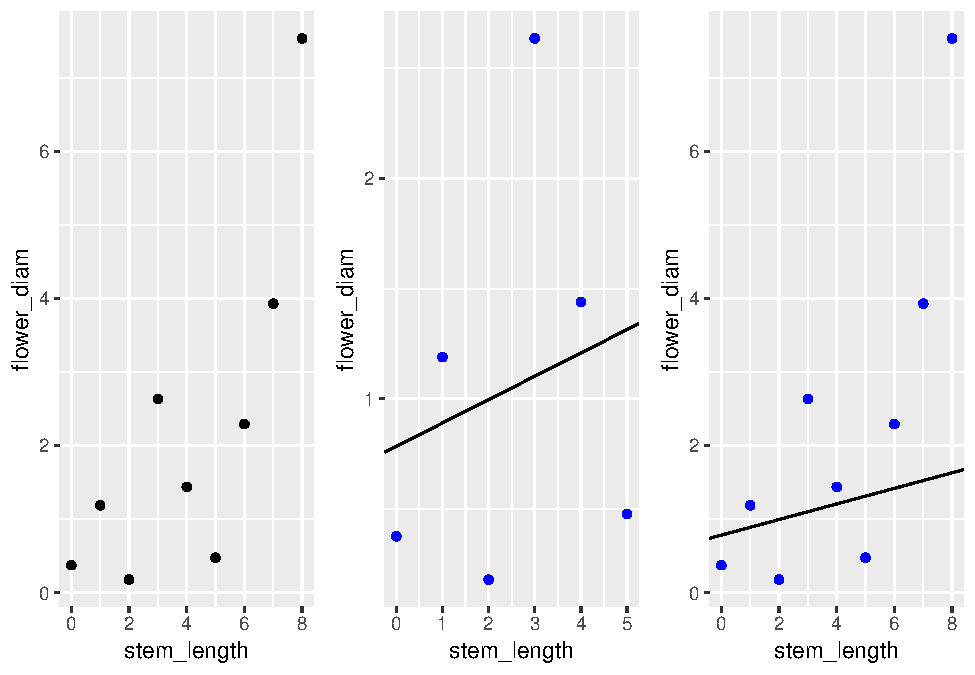
\includegraphics[width=0.9\linewidth]{thesis_files/figure-latex/systematic-1}

Imputation attempts to address this common dilemma in real-world data.
Imputation is the process of replacing missingness in data sets with
some value that redeems the observation for some degree of analysis.
``The aim of these methods is to compensate for the missing data in such
a manner that the analysis file may be subjected to any form of analysis
without the need for further consideration of the missing data'' (Brick
\& Kalton, 1996). Imputation assigns values to missing responses, which
allows records with missingness to be retained during analysis. Ideally,
imputation would eliminate bias in survey estimates caused by ignoring
records with missing data. The catch is that imputation can destroy
intervariable relationships, as well as overestimate the precision of
survey estimates on fabricated data.

There are stochastic and deterministic methods for imputation.
Deterministic regression imputation is the predicted value from a
regression trained on complete-case data. Stochastic imputation differs
due to an additional residual added term to the predicted value, taken
either from a random respondent or comparable observation, and is
usually preferred due to the importance of shape parameters in many
analyses (Brick \& Kalton, 1996).

One traditional method of imputation is the ``Hot-Deck Method'', which
was generally favorable when computation was less efficient. Hot Deck
Imputation requires extensive knowledge of the survey variables in order
to optimize performance since explicit model-based imputation needs a
valid model for every survey variable (Maiti, Miller, \& Mukhopadhyay,
2008). This thesis proposes naive artificial neural networks as a
solution which requires minimal domain knowledge and resists the curse
of dimensionality which other nonparametric methods are susceptible to,
such as local polynomial regression (Maiti et al., 2008).

Due to the difficulties imposed by working with high-dimensional,
complex survey data with varying degrees of domain knowledge, we turn to
neural networks and their structural benefits to reliably perform these
challenging imputation problems.

\chapter{Neural Networks}\label{math-sci}

\section{Introduction to Machine
Learning}\label{introduction-to-machine-learning}
\begin{quote}
From the advent of computation, there has been a drive towards
automation. (Goodfellow, Bengio, \& Courville, 2016)
\end{quote}
The capacity to derive patterns from raw data is known as machine
learning, a broad term for an extremely diverse collection of
algorithms. Machine learning flips the script on classical programming:
whereas classical programming takes rules and data to produce answers,
machine learning creates rules from data and answers by being ``trained
rather than explicitly programmed. It's presented with many examples
relevant to a task, and it finds a structure that derives rules for
automating the task'' (Chollet \& Allaire, 2018).

Machine learning is intended to elucidate or predict patterns in data.
These algorithms handle anything from linear regression for predicting a
numerical response based on a number of features, to clustering for
visualization and assignment of untaught observation classes. Machine
learning models are trained by minimizing error during exposure to
labelled ``training'' data with some underlying distribution and random
noise. After training, models are passed unlabelled ``test'' data to
predict the corresponding unknown class or value. Predictive
(supervised) machine learning algorithms seek to emulate and elucidate a
true unknown generative function from which the data were drawn.

For imputation purposes, our goal will be to accurately estimate missing
values by approximating the generative function from which they are
drawn. Generative functions are of the form \[
y = f(x_1, x_2, \dots, x_n) + \epsilon
\] where the true label \(y\) of the observation is a function of the
features \(x_1, ..., x_n\) perturbed by some random noise \(\epsilon\).

The estimating model will be trained via exposure to labelled
observations, called the training data, then used to predict
observations with missing labels, called testing data. The challenge in
machine learning is learning the correct amount from training data in
order to derive the underlying distribution of the observations without
simply memorizing the labels of the training set. This memorizaion
problem is called overfitting and is central to machine learning.
\begin{figure}
\centering
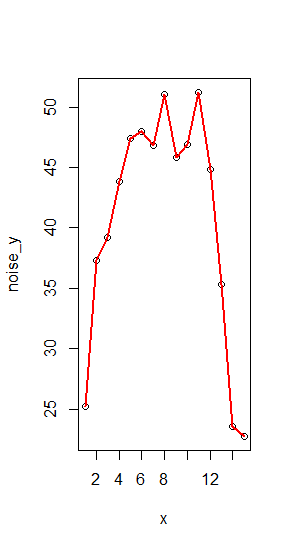
\includegraphics{figure/overfit.png}
\caption{\label{fig:overfit}The overfit model}
\end{figure}
\ref{fig:overfit} is an illustration of this pervasive principle in a
regression example. An overfit (or too-flexible) model simply learns the
observation's labels, rather than the underlying distribution (or
generative function, in this case a second-degree polynomial).

The overfit model \ref{fig:overfit} has extremely low error on the
realization of the data on which it was trained, but fails to learn the
underlying generative function, and instead learns the random noise of
the training observations. Thus this model is a poor descriptor of new
realization from the same generative function, seen in \ref{fig:overfit}
and \ref{fig:overfitre}:
\begin{figure}
\centering
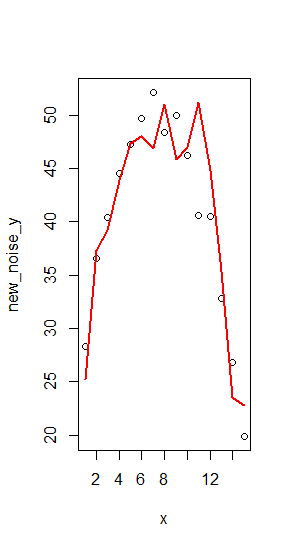
\includegraphics{figure/badfit.png}
\caption{\label{fig:overfitre}Overfit model over new data}
\end{figure}
The overfit model does not accurately reflect the underlying
distribution from which both datasets are drawn. Rather, it captures
only the random noise of the data on which it was trained. It would be a
mistake to assume the generative function is a degree 15 polynomial just
because the training error of such a function is low.

An underfit model, \ref{fig:underfit}, also fails to capture the
underlying distribution, due to a lack of flexibility. A linear
regression, though it minimizes its training MSE, clearly fails to
capture the underlying distribution of the data:
\begin{figure}
\centering
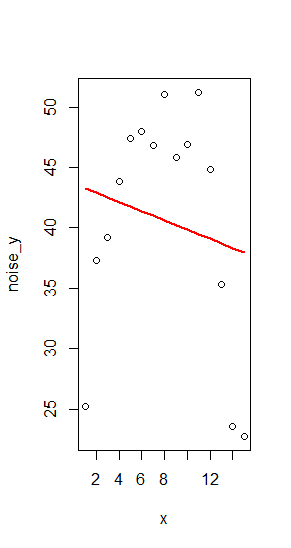
\includegraphics{figure/underfit.png}
\caption{\label{fig:underfit}An underfit model}
\end{figure}
\ref{fig:goodmod} displays a well-trained model which straddles these
extrema and captures the apparent underlying distribution of the data in
a general sense by approximating the generative function from which they
are drawn, and remains fairly constant under different draws from the
same distribution. The aptly-flexible model has consistent performance
on new realizations of the data. The model performing well on data it
was not trained on is called generalizability.
\begin{figure}
\centering
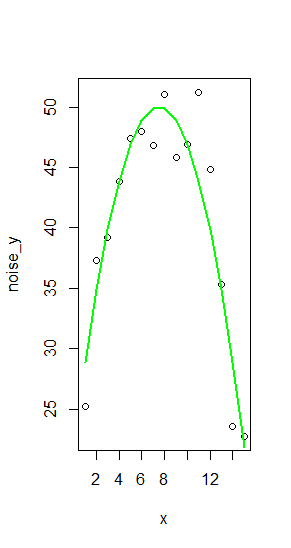
\includegraphics{figure/true.png}
\caption{\label{fig:goodmod}A well-fit model}
\end{figure}
\ref{fig:goodmod} has the correct level of flexibility, and accurately
captures the underlying generative function while avoiding overtraining
based on noise. This makes the model generalize well on a new data draw:

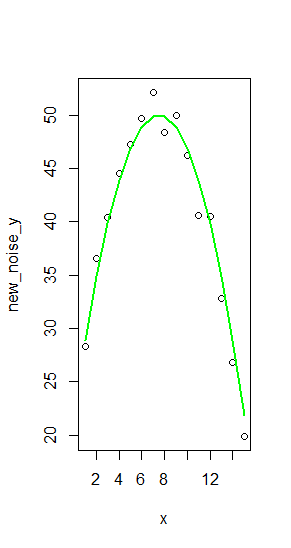
\includegraphics{figure/stayGood.png}

The relationship of the fit and complexity of the model is described by
the bias-variance tradeoff phenomena.
\begin{figure}
\centering
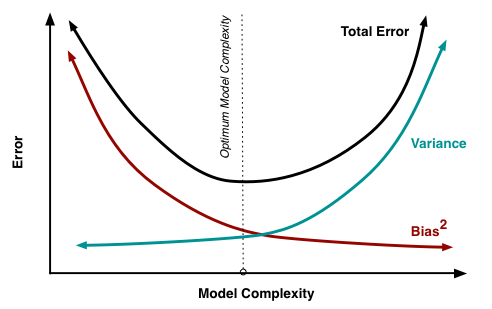
\includegraphics{figure/biasvariance.png}
\caption{\label{fig:biasvar}The bias-variance tradeoff}
\end{figure}
Figure \ref{fig:biasvar}\footnote{Fortmann, Scott. ``Bias and
  Variance.'' Understanding the Bias-Variance Tradeoff, June 2012,
  scott.fortmann-roe.com/docs/BiasVariance.html.} demonstrates the
involvement of model complexity (or flexibility) in terms of training
error. Model complexity refers to the ability of the model to
approximate complex generative functions. We see that as the flexibility
of the model increases, the bias on the training set always decreases,
representing the model's performance on observations with labels.
However, complexity beyond the models optimal value implies
over-flexibility, in which the model is able to memorize random noise
rather than stopping at the trend of the data. This increases the total
error of the model when exposed to data that comes from the same
generative function that the model has not been exposed to, such as a
testing data set or another observation from outside the training set.
Higher flexibility models create more variable models, which though
trained on data from the same generative function differ greatly in
appearance due to the random sample of training data. These models are
unstable for inference and generalize poorly.

One key difference from statistical modelling and survey statistics
methods is the point at which randomness is introduced into the data.
Machine learning attempts to approximate the function from which the
data was randomly generated, while survey statistics imply that
randomness in data comes from the survey design. The paradox of where
randomness is introduced into the data is resolved with the existence of
a superpopulation \(U\), where each observation has label
\(y = f(x) + \epsilon\), some generative function. From this
superpopulation, a population \(u\) is created through \emph{i.i.d.}
realizations from \(U\). From this population \(u\), the survey is
taken. Thus there still exists a generative function from which the
population is drawn, but the features and label of the observations are
fixed by the time the complex survey is taken on the population,
reconciling the two methodologies.

\section{Neural Networks}\label{neural-networks}

\subsection{Background and Context}\label{background-and-context}

Neural networks are a family of machine learning algorithms with an
extended and diverse history of research in neuroscience, statistics,
and computer science. Recently, these models have experienced great
growth in attention and popularity due to the contemporary circumstance
of computational capability. Neural networks thrive on large training
data sets, which have tended to increase in size and availability
throughout time. Neural networks also outperform competing algorithms in
high-dimension feature problems, which are common in real-world machine
learning applications such as image data, waveform data, and large
surveys. Often utilizing derivatives of complex compositions of
functions as an optimization method, deep learning training periods are
computationally intensive, relying heavily on computer hardware and
optimized software for reasonable implementation. Lastly, recent
attention to and development of neural networks can be attributed to
their proven potential in solving complicated real-world applications
with promising and increasingly dominant accuracy in practice, often at
the cost of a lack of inferability.

This lack of inferability is the typical downside of working with neural
networks as the inference on a model can be more important than the
predictive accuracy depending on the problem. Once a simple linear
regression is trained, the coefficients on the predictors offer an
immediately understandable interpretation of the behavior of the data.
For example, a coefficient of .3 on a feature \(x\) has a simple,
instant understanding: as feature \(x\) goes up by 1, the response goes
up by .3. Neural networks however, lack this instant recognition due to
the less intuitive layered structure of input transformations, known as
representation learning.

\subsection{Basics}\label{basics}

Neural Networks are a composition of functions. The following describes
a full neural network:

\[
\hat y = f(\boldsymbol{x}; \theta, \omega) = f^n ( f^{n-1}  ( ... f^1(\boldsymbol{x}; \theta, \omega)))
\] In this function, we see the input features \(x \in \mathbb{R}^n\),
the learned coefficients \(\theta\), the learning rate
\(\omega \in \mathbb{R}\), and the output prediction \(\hat{y}\).
Consider one of the layers of the network, \(f^i\). This layer is an
activation function composed with a linear function:

\[
f^i = \max ( 0 , {\boldsymbol{W}_i}^T \boldsymbol{x} + c_i)
\] Where \(\boldsymbol{W}_i^T \boldsymbol{x} + c_i\) is the interior
linear function for \(\boldsymbol{W}_i^T \in \mathbb{R}^n\),
\(c_i \in \mathbb{R}\).

The activation function shown above is the rectified linear unit, or
\(\max(0,a)\). Activation functions are significant as they introduce
nonlinearity into what would otherwise be a linear function (a
composition of linear functions). \({W_i}^T\) and \(c\) in \(f_i\)
dictate a linear transformation on the input to the layer. An ordered
list of all elements of \(W_i\) and \(c_i\) for all \(i \in n\) would
give the full description of the network, called \(\theta\). So the
output of a 1-layer network can be expressed as

\[
f(x; W, c, w, b) = w^T \max( 0 , \boldsymbol{W}^T \boldsymbol{x} +c ) +b
\]

The final activation function is another structural parameter left to
the designer of the network, but differs from interior activation
functions as the output of the network is restricted to the codomain of
the function, limiting the number of reasonable choices. The typical
output layer for scalar regression is a linear unit, on behalf of the
codomain \((-\infty,\infty)\) of the activation: \[
f^n(\boldsymbol{x}) = 1*(\boldsymbol{W}_n^T \boldsymbol{x} + c_n)
\]

The learning rate \(\omega\) and a loss function are meta-parameters,
given by the user creating the neural network. These two parameters are
used during the training of the network. During training, gradient
descent is used to descend the loss function in order to find the
optimal parameters for the network.

Loss functions are ways of describing the performance of a model when
predicting labels of a data set. The loss function takes the model and
data as inputs, and outputs a real number. Loss functions can be
minimized in training by optimization which leads the network to find
improvements in weights yielding accurate predictions. Loss functions
allow for another degree of customization in the training of a network,
such as in Ridge and LASSO regression. These algorithms add a weighting
to the typical mean squared error loss function which penalizes the
weights on predictors in polynomial regression. These methods introduce
bias into otherwise unbiased algorithms, but reduce the variability of
the model across different draws of data from the same distribution,
aiming to reduce the real test loss and improve the model. The cross
entropy between the data distribution and the model distribution is the
typical choice (Goodfellow et al., 2016).

Cross Entropy: \[
\int_\chi P(x) \log Q (x) dr(x) = E_p [- \log Q]
\]

Take for example the Mean Squared Error cost function: \[
MSE = \frac{1}{n} \sum_{k=1}^n  (y - \hat y)
\]

MSE, a typical loss function for regression applications, takes the mean
squared difference of the predicted label \(\hat y\) and the true label
\(y\) of the observations.
\begin{figure}
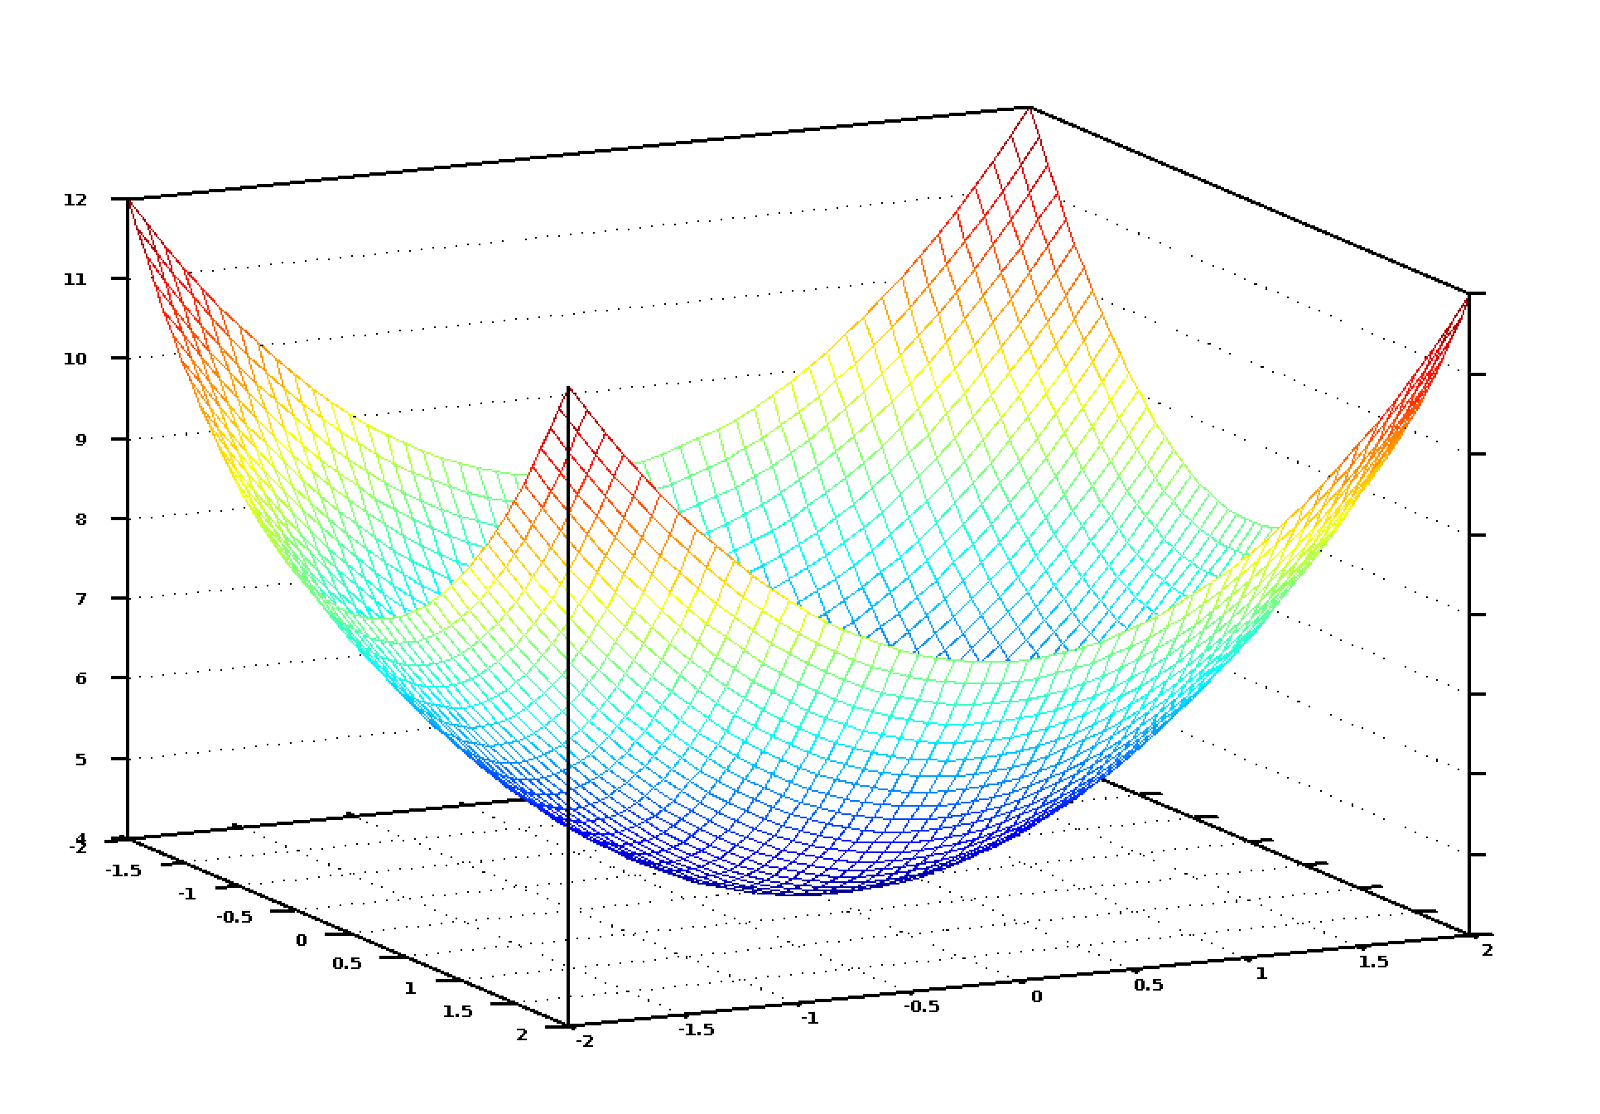
\includegraphics[width=0.95\linewidth]{figure/optimize} \caption{A convex loss function}\label{fig:optimize}
\end{figure}
In \ref{fig:optimize}\footnote{Geitgey, Adam. ``Machine Learning Is
  Fun!'' Medium, Medium, 5 May 2014,
  \href{mailto:medium.com/@ageitgey/machine-learning-is-fun-80ea3ec3c471}{\nolinkurl{medium.com/@ageitgey/machine-learning-is-fun-80ea3ec3c471}}.}
We can see that the loss of a linear regression is a function of \(m\)
and \(c\) given some data which is minimized at \(m = 0\) and \(c = 0\).
The learning rate is the amount that the functions' coefficients are
updated as the loss function is optimized from some initial coordinates
in search of the minimum loss.

Much like training a linear regression, the training of the neural
network aims to drive the approximating function to the underlying
function. The important difference induced by nonparametric models,
however, is the nonconvexity of the loss. The large amount of
coefficients which define even a relatively small network complicate the
optimization problem and make local minima a demanding distraction.
Optimization is typically done with gradient learning using a loss
function, or maximum likelihood estimation. Most modern neural networks
are trained using maximum likelihood, in which the cost function is the
negative log-likelihood between the training data and model distribution
(Goodfellow et al., 2016).

\subsection{Representation Learning}\label{representation-learning}

If you were handed a photograph and were asked if it contained a car,
there's a good chance you would immediately know the answer. But how are
you coming to this conclusion? The human mind recognizes patterns of the
image it has seen before, like a round bumper, a rectangular windshield,
and a few circular tires with a certain spatial relationship to come to
the conclusion that there is, in fact, a car in the photograph. It is
this process of representation learning that prompted early researchers
to create representation-based learning algorithms to extrapolate on
information relationships in the same way as the human mind. The
emulation of human neural cells was the birth of neural networks, a
class of machine learning algorithms which takes its name from multiple
layers of connected nodes simulating a proposed structure of the neurons
of the human mind. Representation learning takes observation's features
as a first layer into a composition of functions, in which each layer
(or function) transforms the data according to a learned representation
transformation that the subsequent layer takes as an input. This
composition allows for complex relationships of features to be learned
in increasingly sophisticated ways, making neural networks ideal for
large-dimensional datasets. For large-dimensional feature spaces such as
in Consumer Expenditure Data, images, or audio, these hierarchical
representations (or layered representations) are important for
distilling human-like feature extraction and iterative predictor space
transformation. To achieve hierarchical representation properties,
subsequent layers understand more complex functions of input variables
as each layer transforms inputs and and weight relationships that
minimize the overall loss of the network. As each layer receives the
transformed output of the previous layer, more complex relationships of
features can be derived.

Successive layers of the network learn transformed representations of
the data which lend themselves to an effective linear regression
performed by the final layer, called the output layer. This process of
successive transformation learns meaningful representations on which the
output layer can be most accurate. Since the full network does not have
a single functional representation, it is nonparametric. The flexibility
and power of neural networks in fields demanding domain knowledge is
that they can approximate any function, per the Universal Approximation
Theorem (Hornik et al., 1989; Cybenko, 1989). The theorem states that a
feedforward network with a linear output layer and at least one hidden
layer with any ``squashing'' activation function can approximate any
function from one finite-dimensional space to another with any desired
nonzero amount of error, provided that the network is given enough
hidden units. Thus the user decision required is the depth and breadth
of the network, optimized through validation set meta-analysis.

Representation learning is extremely important to the broad promises of
neural networks in practice. The basis for this strength is that
subsequent layers of the network learn meaningful structures of the
input data associated with a lower loss score. Correlations of features
forming a functional relationship to the label which induce loss
function descent will be internalized by the composition of subsequent
functions. This property of representation learning is significant for
investigating the necessity of independent and identically distributed
data in deep learning algorithms. Fo survey data, it could be the case
that the significance of the inclusion probability can be learned as a
meaningful feature, with no special tweaks or preprocessing necessary
for the algorithm. Data which require no special tweeks are extremely
meaningful as this circumvents the necessity of incorporating domain
knowledge and expertise in current imputation methods, which holds back
expedient and lightweight research.

These advantages of Hierarchical and Distributed Representation
transformation give neural networks huge advantages in accuracy and
fitting capability for data with a massive hypothesis space. A
hypothesis space is the space of all possible answers to a question.
Image classification, for instance, represents a hypothesis space of
pixels with unknown correlations that must be trained with label
relationships to determine the correct transformative relationsip of
millions of pixels to a most-likely class label. Thus the curse of
dimensionality common throughout machine learning is mitigated through
successive transformation layers.

Neural networks thrive on the interaction of many features, due to the
nature of representation learning which excels in covariate relations
and distilling information encoded between features. Popular modern
applications are image and waveform audio data, in which machine
learning problems become dominated by the Curse of Dimensionality. This
common machine learning problem arises when the amount of data is
insignificant when compared to the hypothesis space or feature space,
and there are sparse observations for some regions. Machine learning
needs many observations with each combination of values, but this
becomes quickly infeasible for data with thousands of features. The
peaking phenomena dictates that there is an optimal number of features
to describe the data before the curse of dimensionality creates
problematic sparsity and dominating observations with few neighbors .
Neural networks are known to resist this commonplace issue due to the
distributed learning property, wherein each node is sensitive to only
particular features.

Distributed representation is a powerful implicit component of neural
networks in which neurons divide feature space to better handle feature
interactions: suppose an image-recognition system could recognize cars,
trucks, and birds, as well as distinguish if these objects are red,
green, or blue. One way of representing these inputs could be to have a
separate neuron for each combination: red truck, red car, red bird, and
so on for nine independent neurons. Distributed representation, however,
could partition these workloads by having three neurons for color and
three for object type. In addition to reducing the number of neurons
required dimensionally, this also distributes the learning demands of
each neuron. The neuron describing redness is able to learn about
redness from any category, not one specific category as the red bird
neuron must (Goodfellow et al., 2016).

Neural networks approximate nonlinear functions by applying linear
models not to the features x, but to a transformed input, \(\phi(x)\),
where \(\phi\) is a nonlinear transformation. \(\phi\) provides a new,
more meaningful representation for \(\boldsymbol{x}\). The question then
is how to choose the mapping \(\phi\):
\begin{enumerate}
\def\labelenumi{\arabic{enumi}.}
\item
  One option is to manually engineer \(\phi\). This takes a huge
  speciality of domain knowledge and practitioner specialization, with
  little transfer between domains. This was the dominant method before
  deep learning (Goodfellow et al., 2016).
\item
  The strategy of neural networks comes from the learning of \(\phi\).
  In this approach, we have a model
  \(y = f(\boldsymbol{x}; \theta, \omega)\) as specified in the neural
  network introduction. Due to the Universal Approximation Theorem, the
  nonparametric deep feedforward network can learn a functional
  approximation from the input to the desired output. This method
  sacrifices the training convexity of the other two, but benefits from
  the genericity of the specifications. The human user need only specify
  a general function family rather than exactly the correct function,
  but can still benefit from designing families of
  \(\phi(\boldsymbol{x}; \theta)\) that they expect to be relevant
  (Goodfellow et al., 2016).
\end{enumerate}
\subsection{Neural Networks for Complex Survey
Data}\label{neural-networks-for-complex-survey-data}

From an optimist's perspective, the need for data preprocessing or
special conditions on the loss function for training the model would be
unnecessary: If learning the correlations and underlying distributions
associated with rare observations from complex survey design would truly
lower the network's loss, it should be learned and accounted for without
the need to perform special external transformations on the data to
``undo'' the effects of complex sample design. For this reason, it is
significant to compare the potentially superior results of a naive model
to one with superfluous data transformations done. A neural network
model with access to an informative \(\pi\) feature ideally would
approximate the function relating the inclusion probability and features
to labels, without the need for extreme domain knowledge and manual
feature engineering.

The optimism of nonparametric algorithms increases in tasks of minimal
domain knowledge and feature engineering capability. Ideally, using
heuristic meta-parameters defining a neural network model would be
enough to get reasonable predictive accuracy in conjunction with one of
the methods of Chapter 3. Per the Universal Approximation Theorem, any
underlying generative function is at worst approximated by a 2 layer
heuristic model, potentially improving upon other naive modeling
procedures such as a weighted linear regression. Additionally, in real
survey data the capacity to derive the significant features from a
high-dimensional space is a weakness of parametric model regression,
which is highly variable in the context of the noisy features explored
in Chapter 4.

\chapter{Methods}\label{methods}

Missingness is an extremely common problem in real data sets. Many
analyses and algorithms such as regression, classification, PCA, and
clustering done throughout the sciences rely on having entirely complete
observations. For this reason, some strategy must be adopted to
transform a raw data set into an analyzable one.

There are multiple approaches for a researcher interested in going about
this process. The researcher has a data set gathered under a complex
survey design where the features \(x_1,...x_n\) and inclusion
probability \(\pi_i\) is known for all \(i\), though the label \(y_i\)
may be missing due to item nonresponse. Sample observations with item
response are the elements \(r \subseteq s\), of which there are \(n_r\),
and there are \(n_{s-r}\) nonrespondents \(s-r \subset s\). In order to
create a data set with no missing values, the researcher may choose to
adopt one of the following methods. These methods borrow notions from
complex survey design about using design variables to model how
characteristics of the population affects the sample (Maiti et al.,
2008). Neural network methods have the advantage of flexibility in
approximating any functional relationship, and can be tuned using
sampling weights to account for complex sampling design using unequal
sampling (Maiti et al., 2008).

There are two primary tasks for a researcher: representative
complete-case data, and statistical estimation via accurate imputation.
The following methods are imputation techniques designed with these
goals in mind. Imputation methods utilize different techniques to create
a complete-case dataset by estimating missing values based on
information from the complete cases. Once the missing values are
imputed, the population parameter is estimated using the approximate
complete-case data set.

\section{Mean Estimation Methods}\label{mean-estimation-methods}

\subsection{Naive Mean}\label{naive-mean}

A common statistic of interest to a researcher is an estimate of the
population mean \(\mu_y = \frac{1}{N}\sum_{i \in N} y_i\) using the
information from the complex sample with missingness. Taking the naive
mean of complete cases is insufficient for two reasons. The first has
been discussed in Chapter 1, which is the potential of systematic
missingness in the data. The second is that the naive mean makes the
assumption that the observations represent equal proportions of the
population, as in an \emph{i.i.d.} sample.

The naive mean estimator ignores survey design and allows equal
contribution of all observations: \[
\hat \mu_y = \frac{1}{r} \sum_{i \in r} y_i
\]

\subsection{\texorpdfstring{\(\pi\)-Corrected Naive
Mean}{\textbackslash{}pi-Corrected Naive Mean}}\label{pi-corrected-naive-mean}

We resolve this issue in the mean estimate formula by weighting
contributions to the mean by \(\frac{1}{\pi_i}\), the approximate number
of population members represented by observation \(i\). This value is
the Horvitz-Thompson estimator of the true number of people who would
respond in the population (Horvitz \& Thompson, 1952): \[
\hat \mu_y = \frac{1}{\hat N_r} \sum_{i \in r} y_i \frac{1}{\pi_i}
\] Where \(\hat N_r = \sum_{i \in r} \frac{1}{\pi_i}\). This resolves
the problem of ignoring the survey design in estimation, but does not
account for systematic bias resulting from missingness. For example, the
\(\pi\)-corrected naive mean estimate of the population mean will be an
under-estimate of the true population mean in the presence of systematic
missingess of large observations.

Let \(\hat \mu_y\) be the sample estimate of the population mean
\(\mu_y\). The oracle mean can be considered the ``best estimate'' of
\(\mu_y\), but it is only available in simulation. The oracle mean uses
information that the simulation manually drops so as to create an ideal
population estimate given a survey sample:

\section{Imputation Methods}\label{imputation-methods}

In order to combat the presence of systematic missing values, we utilize
imputation to label the missing observations with the best estimate of
\(y_i\), \(\hat y_i\). Imputation has the added benefit of approximating
a complete-case dataset without dropping observations.

\subsection{Imputation Mean Estimator:}\label{imputation-mean-estimator}

\[
\hat \mu_y(\text{method}) = \frac{1}{\hat N} (\sum_{i \in r} \frac{y_i}{\pi_i} + \sum_{i \in s-r} \frac{\hat y_i}{\pi_i})
\] Where \(s-r\) are the missing cases, \(r\) are the respondents, and
\(\hat N = \sum_{i \in n} \frac{1}{\pi_i}\) is the Horvitz-Thompson
estimator of the population size (Horvitz \& Thompson, 1952).

\subsection{Drop NA}\label{drop-na}

One option is to simply remove the observations with missing labels from
the data set. This method is extremely easy to implement and serves as a
sure-fire way to end up with a data set with no missing values. There
are two downsides to this method: The first is that removing
observations with missingness obviously decreases the size of the data
set and can nontrivially reduce the fidelity of models aiming to
understand the population from which the data was taken. The second
problem is the assumption of random missingness. If there is any
correlation of label to amount of missingness, systematic bias is
introduced into the data set, as discussed in Chapter 1. For example, if
there is a possibility that larger values are more likely to be dropped,
then as a result the sample mean would underestimate the population
mean.

\subsection{Median Imputation}\label{median-imputation}

Median imputation is another easy way to get complete cases in data for
analysis or estimation. Median imputation simply fills in the missing
labels with the median of the respondent labels. Median imputation has
multiple problems for analysis or estimation. The median offers equal
weighting to all observations in a data set, meaning it destroys the
informativity of the inclusion probability \(\pi\). It also removes
correlation of feature and label, making analyses such as PCA less
informative, as covariate relations dictate axis derivations. Median
imputation is extremely fast to execute and implement, but creates
noninformative observations in the same manner as the Drop.NA method.

\subsection{Weighted Linear Regression Imputation}\label{sec:linear_reg}

Linear regression is a convex optimization problem of \(p+1\)
parameters, where \(\hat f(x) = \hat y = (m_1x_1 + .+ m_px_p)+b\) is the
estimate of \(y\) for observation \(i\) given features
\(\boldsymbol{x} = [x_1, \dots ,x_p]\). Using the mean of the squared
difference between the predicted and actual responses of a training data
set, weighted-MSE linear regression scales the squared error
contribution of each observation by \(\frac{1}{\pi_i}\) to account for
rare-case observations with potentially systematic missingess, and
returns a scalar loss: \[
\text{MSE}(f) = \frac{1}{\hat N} \sum_{i \in r} (\frac{1}{\pi}(\hat{y} - y))^2 \label{eq:wmse}
\] Significant to this algorithm, however, is the contribution of
\(\pi\) regardless of whether it is informative. In data known to have
systematic label missingness, this is not a problem. However, it is not
always the case that \(\pi\) is informative, and including this scaling
term would be harmful to cases in which \(\pi\) and \(y\) are
uncorrelated.

\subsection{Naive Neural Network
Imputation}\label{naive-neural-network-imputation}

Neural Network Imputation is our baseline model for imputation for
estimating a population mean. The number of hidden layers, nodes, and
loss is left to the user, which would be an incorporation of domain
knowledge or exploratory modelling to derive a reasonable model load for
learning the data's generative function. In the context of the
researcher having minimal knowledge of the data, a neural network with 2
hidden layers of 32 units activated by \texttt{relu} functions is a
reasonable starting point. Overtraining due to overflexible models can
be stimied with a validation set, assuming the data is not so small as
to create unrepresentative data by subsetting the training data further
(\(n > 10^3\)). ``Naive'' neural network imputation refers to this model
not having access to the \(\pi\) feature of the observations as a
predictor or incorporate it in any way. This model uses the assumption
that the data is \emph{i.i.d} as a representative for ignoring the
survey design, an assumption which is known to be a significant problem.
Regardless, the neural network should approximate the generative
function with some nonparametric fit, but underestimate the population
mean as a result of systematic missingness and observation equity. This
baseline model will be the pacemaker for the other neural network
methods to improve upon by incorporating survey design information.

\subsection{Weighted Loss Neural Network
Imputation}\label{weighted-loss-neural-network-imputation}

Weighted Loss Neural Network Imputation takes inspiration from the
weighted linear regression algorithm. This neural network training uses
the same \(\pi\)-weighted MSE of @ref(sec:linear\_reg), but sacrifices
the convexity of the loss function of the linear model, which means
pervasive local minima which are distracting to the learning algorithm:
\[
\text{MSE}(f) = \frac{1}{\hat N} \sum_{i \in r} (\frac{1}{\pi}(\hat{y} - y))^2
\] The existence of local minima from the high-dimensional model space
comes from the flexibility of the many hidden neurons weight
transformations within the model. A loss-weighted neural network hopes
to account for systematic missingness in the data by heavily punishing
the loss term generated from rarer observations. Since rare observations
are more likely to be missing, they must be given more weight since they
appear less in the training data then the population. Thus a weighting
scheme attempts to un-do systematic missingness by making the rarer
observations as ``heavy'' as they would be in the true population by
making outliers be worth multiple observations to the loss contribution.

\subsection{\texorpdfstring{\(\pi\)-Feature Neural Network
Imputation}{\textbackslash{}pi-Feature Neural Network Imputation}}\label{pi-feature-neural-network-imputation}

A \(\pi\)-feature neural network has access to \(\pi\) as a predictor
during training and testing. This is a realistic assumption to make as
data collected under a complex survey design must have a \(\pi\)
probability regardless of whether the label is missing. This method has
the benefit of adapting to whether \(\pi\) is truly correlated to \(y\),
which the loss-weighted method assumes. A neural network optimist could
claim that if there is a significant relationship of \(\pi\) to \(y\),
it will be reflected in the loss during training and the network will
adapt accordingly to the information provided by the feature. However if
\(\pi\) and \(y\) are uncorrelated and the missingess is random, the
network will not still weight the observations and will correctly ignore
the feature to create more accurate predictions with no need for domain
knowledge on the relationship of the missingness.

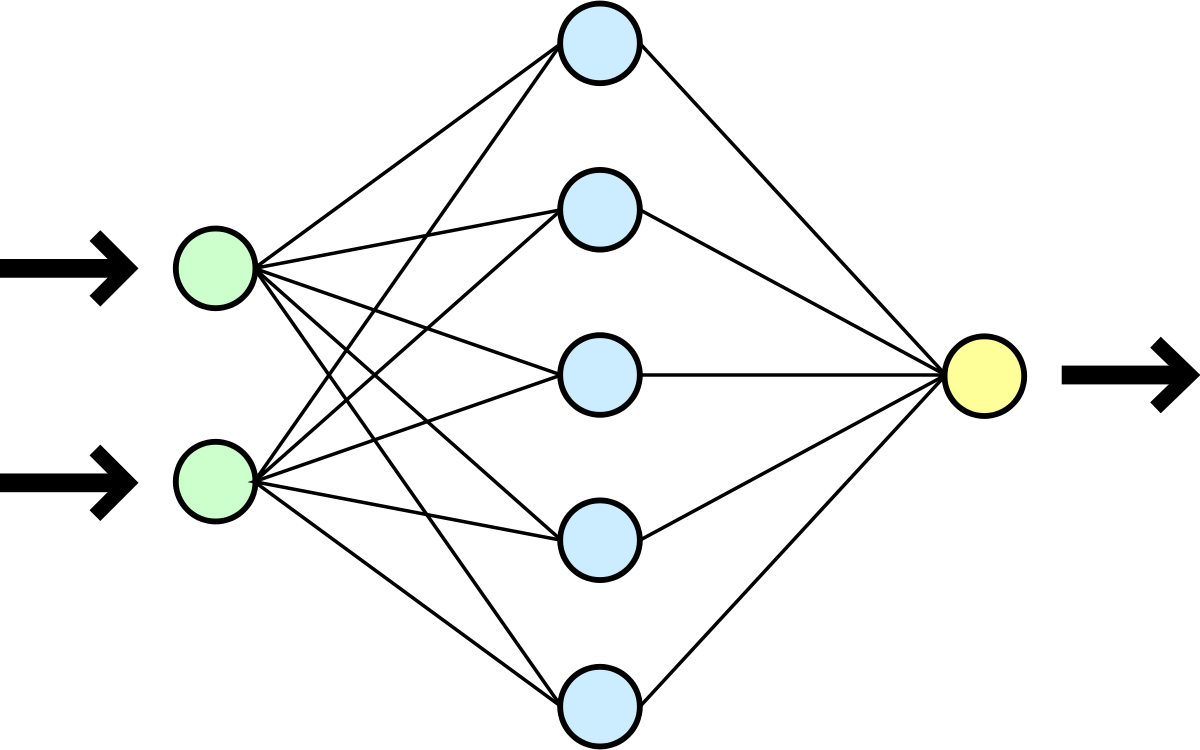
\includegraphics[width=0.8\linewidth]{figure/network}

\subsection{Weighted Resample Neural Network
Imputation}\label{weighted-resample-neural-network-imputation}

The weighted resample method uses the same model as the naive neural
network imputation but uses a data preprocessing step to incorporate the
survey design information. A weighted resample of size \(n\) is taken
from the sample with replacement with observation selected by
probability \(\frac{1}{\pi}\). The inference of this method is an
attempt to ``undo'' the effects of survey design in gathering the data.
A weighted resample in which observations are selected by the inverse
inclusion probability uses the insight that an observation with
inclusion probability \(\pi\) represents \(\frac{1}{\pi}\) members of
the population. By sampling on this probability, the resampled data set
should be an estimate of an \emph{i.i.d.} sample from the population,
making it viable for supervised learning ignoring the survey design
elements. From this point the naive neural network method is applied
(and directly compared to naive neural network estimates), since ideally
this is \emph{i.i.d} data without need for survey design information
tweaks on the algorithm.

\subsection{Derived Feature Neural Network
Imputation}\label{derived-feature-neural-network-imputation}

This method pre-processes the data by adding additional features to the
data. In the simulation and \texttt{CE} experiments, this is done by
multiplying two informative features with \(\pi\) and concatenating the
result to the data. The intention of this method is expediting the
training process to allow the approximation of more complex generative
functions with less model capacity and training. Intuitively, should the
relationship of \(\pi\) to \(x_i\) in the missing data be relevant, it
will be more easily learned for superior prediction accuracy. This
method does have an implicit ``oracle'' element, however, as knowing
which columns to derive from a real data set is incorporation of a
significant amount of domain knowledge.

\chapter{Simulation}\label{simulation}

\section{Exploration of Methods Using
Simulation}\label{exploration-of-methods-using-simulation}

Simulated data is used to evaluate the methods in order to get an
understanding of their performance on a data set with known
characteristics.

Full insight into the feature distributions, generative function, random
noise, and systematic missingness allow for controlled experimentation
on when certain methods thrive. Simulation allows for parameters such as
label noise and feature informativity to be changed and measure the
response of the methods across any domain.

\section{High-Dimension Simulation}\label{high-dimension-simulation}

Often in real-world data, there might be a large number of features, not
all of which are necessarily correlated to the response label. For
example in the Consumer Expenditure data, age, gender, ethnicity, and
education might have a predictive relationship with household income,
while a number of others such as state, reference person gender, and
social security income may not. The ability for a model to discern which
features are relevant and which are not is a significant benefit both
for inference and predictive consistency. Inspired by research in best
feature selection methods, non-correlated features are used in the model
evaluation step in an attempt to more realistically simulate complex
data (Hastie, Tibshirani, \& Tibshirani, 2017). The addition of these
features contributes to the curse of dimensionality and variability of
estimates.

These additional ``noisy'' parameters are simulated by making the
generative function of the labels \(y\) not a function of some of the
features. All methods used in the simulation are accompanied by their
oracle counterparts, meaning the same method is run two times: one with
access to all features, the oracle restricted only to the relevant
features which are inputs to the generative function.

\section{Monte Carlo Simulation}\label{monte-carlo-simulation}

Monte Carlo (MC) simulation attempts to overcome the inherent randomness
of sampling and model training by repeated iterations of the sampling,
training, and evaluation steps. A distribution of output estimates is
made over many potential samples from the population in order to get a
more complete interpretation of the results.

It should be noted that neural networks can be more optimized than in
their performance in the following simulation study. This is because a
network can be intentionally over-trained on the training data, then
re-trained from scratch to the number of epochs which minimized the
validation loss. This poses a challenge in MC simulation, however, where
many iterations without user input are needed. Additionally, runtime
becomes a vastly greater concern when networks must be over-trained
through many epochs, more than doubling the execution time. If
computation were no expense, the neural network methods could be
expected to be slightly more accurate than the below results. This is
somewhat mitigated by a weighted sampling scheme with somewhat low
observation variability and a strong signal between features and label.

\section{Creating a Simulated
Population}\label{creating-a-simulated-population}

The size of the population is \(N=10^5\) and the sample is \(n=10^3\)
observations. Despite neural networks thriving in higher-dimension
settings (both of features and observations), complex surveys are often
implemented on real data with scarce observations, making a lower-size
simulation more suitable for generalizability.

The features simulated population is made as the first step of the
process. Two informative features \(p_1, p_2\) are drawn from random
uniform distribution: \[
f(x) = \frac{1}{30+30} \text{ for } x \in (-30, 30)
\] In addition to two informative features, there are \(20\)
uninformative features drawn from the normal distribution. This
distribution is arbitrary but can have unintended consequences due to
accidental correlation, noted in \{Hastie et al. (2017)\}.

The population labels \(y\) are a nonlinear function of the informative
features: \[
y = p_1^2 + p_2^2
\] The labels are then made nonpolynomial by contorting the parabola
into a ``bowl with flat lip'': \[
y' = \left\{ \begin{array}{cc} 
                y & \hspace{5mm} y<\bar{y} \\
                \bar{y} & \hspace{5mm} y \geq \bar{y} \\
                \end{array} \right.
\]

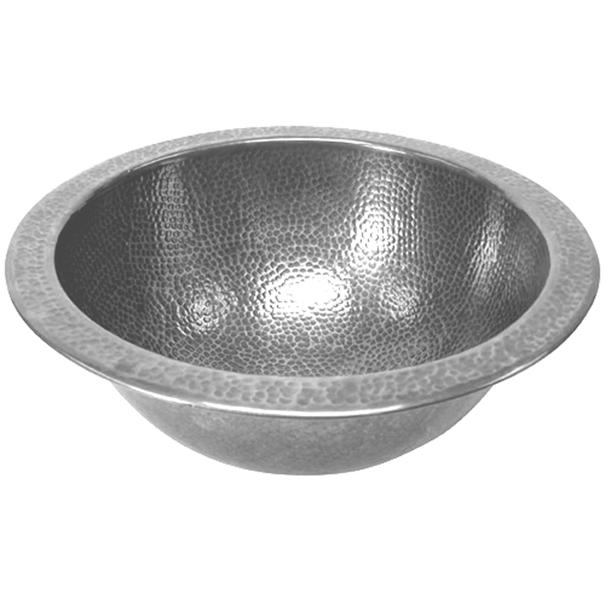
\includegraphics[width=0.7\linewidth]{figure/bowl}

Random noise \(\epsilon\) with \(\sigma = 1\) is then added to the
transformed labels: \[
y'' = y' + \epsilon_y
\]

An inclusion probability \(pi\) is then assigned to each observation
with a strong correlation to \(y\), as well as random normal noise with
\(\sigma = 1\): \[
\pi = \sqrt{y''} + \epsilon_\pi
\] These values are then rescaled to (0,1) and rescaled so
\(\sum_i^N \pi_i = n\).

Combining the information \(y,\pi, p_1, p_2\) and uncorrelated features
gives the population on which the simulation will be performed. The true
mean of the population labels \(\mu_y\) is now known and recorded.

The Monte Carlo simulation is performed for 100 iterations. This is a
low number of trials, but is constrained by the computation intensity of
running 10 neural networks trained for hundreds of iterations each, as
well as performing many weighted samples.

Within each iteration, a single estimation procedure is performed.
First, a weighted sample from the population is taken with respect to
the inclusion probabilities \(\pi_i\) on each observation. From this
sample of \(n=10^3\) observations, an oracle data set is made by
dropping the noise columns, keeping only \(p_1, p_2, \pi,\) and \(y\).
This data set will be used as a benchmark to mirror each imputation
method in order to gauge the potentially harmful effects of
uninformative features common to real data.

The first step is to record the oracle mean, calculated using
information the other methods are not privy to: \[
\hat \mu_{\text{oracle}} = \frac{1}{n} \sum_{i=1}^n y_i \frac{1}{\pi_i}
\]

All subsequent methods are the methods of study, to be performed where
there is missingness in the data. \(20\%\) of the observations manually
have their labels dropped weighted by \(y\), so large labels are more
likely to be absent. The result is the form of data we are using to
simulate method performance: a complex sample taken from a population
with some kind of systematic bias in item response.

The \(\pi\)-corrected mean estimate, weighted linear regression, and
median imputation methods are all described fully in chapter 3, and are
closed-form algorithms with no randomness in the fitting and estimation
processes. The neural network models, however, have a much larger degree
of flexibility and randomness involved in the implementation and
execution of the estimate during simulation making monte carlo
variability more pronounced.

Neural networks are trained using normalized data on non-convex loss
curves in high-dimensional space, making their optimization process
stochastic. This simulation uses the heuristic \texttt{adam} optimizer.
Each model in this simulation uses a 2 hidden layer network with 32
hidden units per layer to make results and applications more comparable.
Each layer is wrapped in the \texttt{relu} activation function: \[
\text{relu}(x) = \max(0,x)
\] The breadth and depth used here is a heuristic size which could
potentially be optimized to suit the problem. This, however, creates a
conflict of interest with information leakage which the other methods
are not privy to, which induces bias for the success of these
algorithms. To maintain the narrative of a minimal-knowledge naive fit,
these models use a reasonable exploratory capacity. The models in the
fitting process are manually over-trained, then re-trained from scratch
to an optimal state. This is done using a validation data set of
\(15\%\) of the training data. Once trained to an approximate loss
minima, the models predict on holdout test data (the observations
missing labels) and the population mean estimate is computed and
recorded.

\section{Evaluating models}\label{evaluating-models}

\subsection{Oracle Mean:}\label{oracle-mean}

The oracle mean is the Horvitz-Thompson estimator with access to the
complete sample before missingness is induced (Horvitz \& Thompson,
1952). The oracle mean will be used as a benchmark against which the
other methods will be compared. \[
\hat \mu_{\text{oracle}} = \frac{1}{N} \sum_{i=1}^n y_i \frac{1}{\pi_i}
\] Since the oracle mean has access to information that the other
methods do not, it is the ideal estimate of a population mean given a
sample. The difference between the oracle and \(\pi\)-corrected
estimates are indices \(n\) and \(r\) over which the sum is taken.

\section{Results}\label{sim_results}

Not a place to list findings. Rather, convince that what I did is
correct, worthy of study, and impactful. Be honest about the
generalizability of the work. If the findings are negative, take care to
explain why the results still matter (discussion of why linear
regression is so dank at mean estimation). Cast the negative result as a
useful insight, rather than a problem with the methodology.

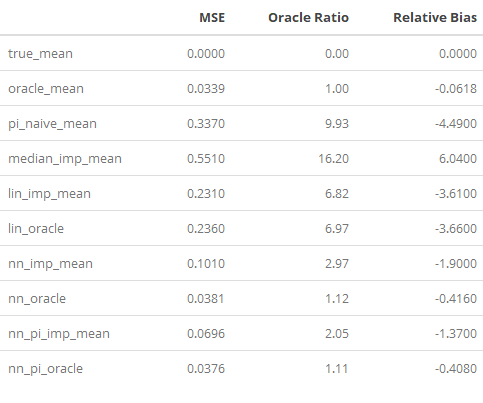
\includegraphics{figure/AWS_results.png}

The weighted-MSE and derived-parameter methods were left out of the
simulation results for runtime concerns and unpromising results on this
generative function.

The oracle counterpart for each method outperforms the noisy-parameter
method, as is expected. The discrepancy in the linear regression method
can be attributed to monte carlo variability, but the finding is
significant that these are so similar. Whereas the neural network
methods were anticipated to have consistent results despite noisy
parameters while the linear regression would struggle, the opposite is
true. This could be attributed to the training duration, as a higher
number of epochs may have dropped the weights of the noisy parameters to
be ignored.

All methods underestimated the population mean, described by the
relative bias column of the results. EXCEPT FOR MEDIAN????? WHAT?????
HOW IS MEDIAN IMPUTATION OVER ESTIMATING! This is reasonable on behalf
of the systematic missingness of the data, but each non-naive method
attempted to mitigate this amount. The results indicate that the
negative bias was significantly larger for non-oracle methods, meaning
noisy parameters could contribute to mean under-estimation. For this
reason, a researcher with some level of domain knowledge should
hand-select features known to have a relationship to the label to be
used as training data, rather than including all available features.

In the case of a nonlinear generative function with little noise, it
should come as no surprise that most nonlinear neural network methods
outperformed the linear.

The \(\pi\)-feature neural network's fantastic performance can be
largely attributed to the significant relationship of \(\pi\) to the
label \(y\): \(\pi = \sqrt{y} + \epsilon\). This strong relationship is
not unreasonable, however, as the positive correlation of inclusion
probability to label is known to occur in real-world data on
salary-related data across BLS business surveys.

Despite a highly nonlinear generative function, the nature of weighted
linear regression is highly successful for mean estimation. In the
context of the bowl-with-lip shape generative function, the linear
regression looks like a flat plane relative to the \(x_1, x_2\) axes
slightly above halfway up the bowl. This is an unfortunate side effect
of the parabola-shaped true function, as the label predictions of the
linear model are bound to this plane. A more realistic nonparabola
context would lend itself to considerably more successful linear
imputation estimates, as the weighted high-label outliers would be
properly represented by the plane's extrema on the domain.

When estimating the population mean, accurate imputation results do not
factor into the score. Rather, the mean of the distribution of imputed
labels solely defines the score of the algorithm. In the case of mean
estimation, linear regression provides an extremely lightweight
estimation method in terms of computational time and implementation that
cannot overfit to the respondent data. Though among the largest MSE
ratios, linear regression should be considered a success in this
experiment and taken seriously as the imputation method to beat.

\chapter{Consumer Expenditure
Surveys}\label{consumer-expenditure-surveys}

\section{Data}\label{data}

The Consumer Expenditure (CE) Surveys\footnote{\url{https://www.bls.gov/cex/pumd-getting-started-guide.htm}}
provide data on ``expenditures, income, and demographic characteristics
of consumers in the United States. The CE data are collected by the
Census Bureau for the Bureau of Labor Statistics (BLS). The data are
primary used to revise the relative importance of goods and services in
the market basket of the Consumer Price Index''.

The data will be the \texttt{fmli171x} survey data, one of the quarterly
surveys for 2017 which contains household information such as specific
incomes, expenditures, home description, and family description. The
data has a low degree of missingness as quarterly information is
propagated between surveys to create complete observations.

The mean estimation methods from chapter 3 will be used to estimate the
population mean household income before tax, \texttt{FINCBTAX}. Like all
data gathered by BLS \texttt{FINCBTAX} is subject to missingness, but
has been imputed in their data sets. This means for the purpose of our
experiment on method imputation quality, we must artifically impose
missingness then compare our imputation results to a combination of true
labels and BLS-derived labels. This is an unavoidable pitfall of working
with real data, as we paradoxically require ``truly missing'' labels to
impute, but need the true label to compare the quality of our imputation
to.

According IRS Statistics of Income, the average household adjusted gross
income (AGI) was \$67,565 in 2015. This is the last year the population
mean household income is available. This numbercould be considered the
true population mean \(\mu_y\), but is derived differently than the BLS
CE data.

\section{Procedure}\label{procedure}

The CE data method performance comparison will be performed in much the
same way as the simulated data method comparison.

The \texttt{fmli171x} survey data is first pre-processed to remove
features with large swathes of missingness. For this study, features
with more than 33\% missing values are dropped from the data set.
Features with missingness less than 33\% are then median-imputed, where
missing values are replaced with the median value of the feature. The
median in this case is used for reasons: it returns only reasonable
values, is uninformative, and does not rely on multiple imputation.

The label to be used is \texttt{FINCBTAX}, the financial income of the
response household before taxes. This label has no missingness as it is
BLS-derived (already imputed).

This process returns a complete-case data set of 6208 family samples
across 607 variables. There are 127 million households in the US, whcih
can be used as an approximate population size \(N\).

The problem of assessing model performance in real-world data is the
paradox of missing labels: ideally, we would impute a missing label,
then learn the true value, and score the model accordingly. For this
data, we will again rely on Monte Carlo simulation to create a
distribution of population mean estimates (U.S. mean household income)
by inducing missingness in the known labels, imputing, and comparing
results via MSE to the true mean.

The following process is repeated a number of times to create a
distribution of mean estimates for each method: 1. Record the true
(sample) mean and Horvitz-Thompson mean estimate 2. Induce missingness
on 20\% of the labels, weighted to larger labels 3. Perform and record
each model's mean estimate + For the real data, a more accurate neural
network method is adopted in which each network undergoes two trainings:
the first finds the ideal train duration by overtraining on the training
data, the second re-trains the model to the validation minimum of the
first model. 4. The results are compared using MSE, oracle ratio, and
PRB.

The dimension of the neural networks has changed somewhat to account for
the new data. Since the number of informative parameters has increased
along with the complexity of the generative function transforming them
to the label, the size of the model has increased. The standard
real-data neural network uses the same two hidden layers activated by
\texttt{relu} and a linear output layer, but now has 64 hidden units per
layer. This describes a significantly higher dimension model as the
input vector \(\boldsymbol{x}\) undergoes multiple high dimension linear
transformations wrapped in the \texttt{relu} activation: \[
\boldsymbol{x} \in \mathbb{R}^6 \\
\rightarrow \mathbb{R}^{64} \\
\rightarrow \mathbb{R}^{64} \rightarrow \mathbb{R}
\] Parameterized by matrices of dimension \(6 \times 64\),
\(64 \times 64\), \(64 \times 1\), instead of \(6 \times 32\),
\(32 \times 32\), \(32 \times 1\) as in the 32 hidden unit simulation.

To accomidate the significantly higher number of trainable features in
this network the hyperparameter \(\omega\), the learning rate, must be
initialized higher in the \texttt{adam} optimization algorithm. This can
expedite the number of epochs (training data exposures) needed for the
algorithm to converge, but can sacrifice predictive fidelty, a
constraint imposed by computational demand. This tradeoff is made in the
name of a more statistically informative monte carlo simulation.

\section{Results}\label{results}

Not a place to list findings. Rather, convince that what I did is
correct, worthy of study, and impactful. Be honest about the
generalizability of the work. If the findings are negative, take care to
explain why the results still matter. Cast the negative result as a
useful insight, rather than a problem with the methodology

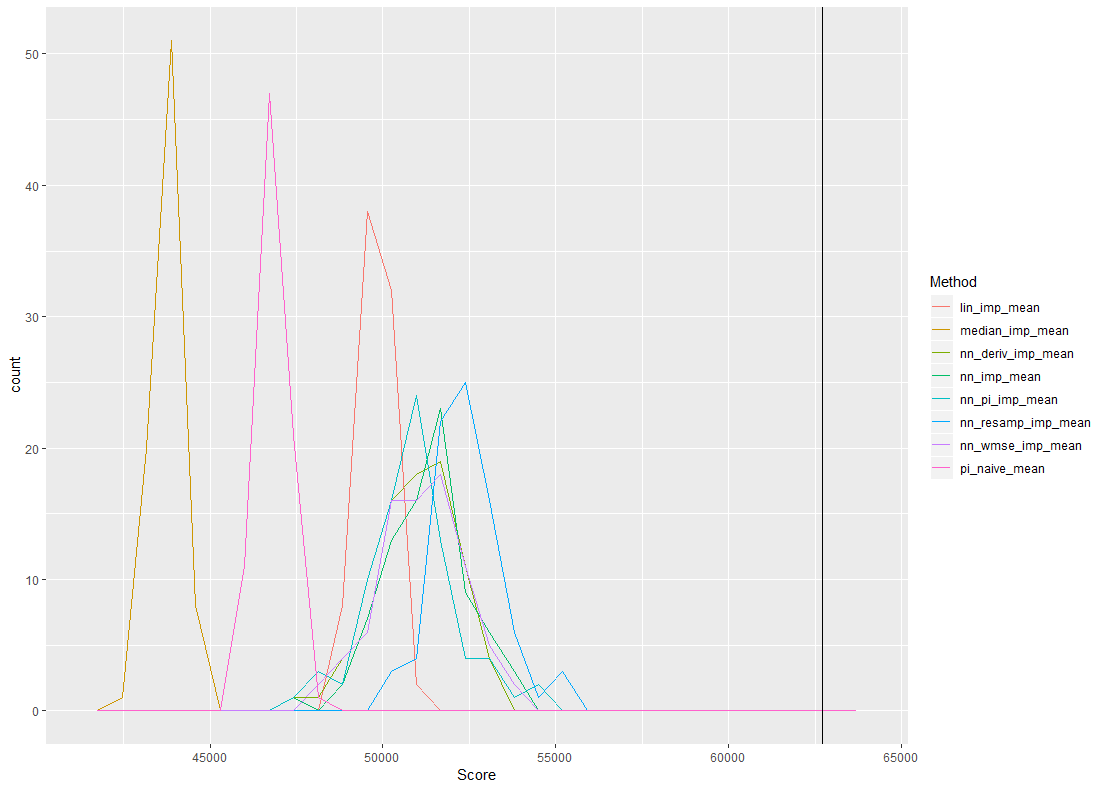
\includegraphics[width=0.7\linewidth]{figure/vline_fig}

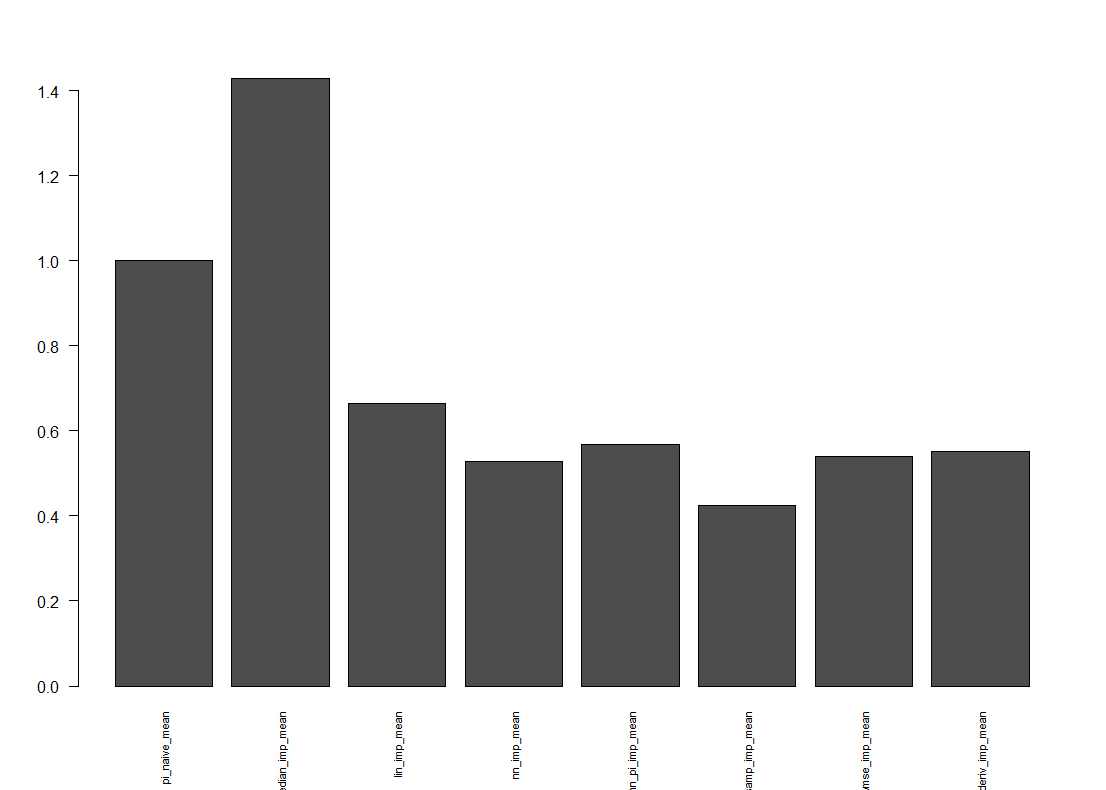
\includegraphics[width=0.7\linewidth]{figure/new_bar_results} From an
ultra-early glimpse (iterations = 5), resample is best. Really cool
stuff, especially considering 1. resample was terrible in simulation and
2. resampling to n didnt seem like a good idea. But its performing great
so far. super cool. all the methods are really, really far off.
estimating 50k when true is 62k. But NN seem to be on-par or slightly
outperforming linear sometimes. we'll see how it shapes up

\chapter*{Conclusion}\label{conclusion}
\addcontentsline{toc}{chapter}{Conclusion}

If we don't want Conclusion to have a chapter number next to it, we can
add the \texttt{\{-\}} attribute.

\section{The End}\label{the-end}

the end of the paper should summarize your main finginds, interpret what
your results mean in context, discuss limitations, and point to where
there is room for4 improvement or further analaysis. This is your last
chance to make an impression, and say everything I want to say.

\section{Discussion}\label{discussion}
\begin{enumerate}
\def\labelenumi{\arabic{enumi}.}
\tightlist
\item
  What are the key features of your analysis and results?
\item
  Do your results confirm or contradict your initial expectations or
  earlier work?
\item
  What problems did you run into, and if still unsolved, wgat are
  suggestions for addressing
\item
  Knowing what you know now, what reccomendations in context do you
  have?
\item
  What should someone work on next, building off of your work?
\end{enumerate}
conclsuion can talk a lot about the TONS of hyperparameters, all the
caveats - can slap a basic version of NN on without domain knowledge,
but can incorporate knowledge in tons of tweaks on all the
hyperparameters

\section{Conclusion}\label{conclusion-1}

A conclusion should not introduce new material. Conclusion brief, and
only contain main points of paper. It will be redundant: that is the
point.

If a researcher is interested in an easy to implement, computationally
inexpensive heuristic algorithm to impute complex survey data for mean
estimation, weighted linear regression is the most appealing method. The
reality of real data is that it is more likely noisy than functional.

The performance of linear regression in noisy-feature simulation shows
the robustness of the algorithm to heuristic implementation. The lack of
domain knowledge necessary to select variables in order to implement an
effective linear regression makes the model highly appealing for stable
results regardless of feature space size.

Neural network methods are promising, however, because of their many
degrees flexibility. The nonparametric models are adaptable to more
complex intervariable relationships of the data. If a domain expert
hypothesized a sophisticated function on a subset of variables which
make an excellent label predictor without knowing its specific form,
there is room for that structure in the neural network architecture.

Likewise, the massive space of hyperparameters for even a simple
feedforward neural network gives immeasurable potential to a savvy
designer. Understanding of the shape of the loss function, necessary
load of the model, and relationship of features are all examples of
knowledge lending itself to specific selections of model load,
activations, optimizers, losses, weightings, connectivity, and countless
other tweaks letting a knowledgable designer maximize predictive
performance.

However, as mentioned in @ref(sec:sim\_results), the task is population
mean estimation, not predictive accuracy. {[}{[}{[}{[}{[}{[}{[}Talk to
kelly about this. obviously predicting values near true label is good,
but that need not be the case to get extremely accurate population
estimates{]}{]}{]}{]}{]}{]}{]}

\section{Future Work}\label{future-work}
\begin{itemize}
\item
  something better than linear regression as comparison: local
  polynomial, etc. some other very-stable heuristic method
\item
  re-visiting weighted resampling by trying bootstrapping methods,
  bigger resample. bootstrapping many datasets, training on each, and
  taking mean of estimates. somethign like this to stabilize predictions
  and sampling variability.
\end{itemize}
Multiple imputation: since hopefully NN preserve intervariable
relationships better than linear or median etc

\appendix

\chapter{The First Appendix}\label{the-first-appendix}

This first appendix includes all of the R chunks of code that were
hidden throughout the document (using the \texttt{include\ =\ FALSE}
chunk tag) to help with readibility and/or setup.

This appendix contains every line of code necessary to replicate the
results of the two experiments detailed in this thesis. The bulk of each
experiment is testing structures used to derive optimal runtime and
epoch-time for each of the many methods, and evaluate their performance
across a variety of standards, seen at the end of each iteration loop.

\section{Data Processing}\label{sec:data_process}
\begin{Shaded}
\begin{Highlighting}[]
\CommentTok{# This chunk ensures that the thesisdown package is}
\CommentTok{# installed and loaded. This thesisdown package includes}
\CommentTok{# the template files for the thesis.}
\ControlFlowTok{if}\NormalTok{(}\OperatorTok{!}\KeywordTok{require}\NormalTok{(devtools))}
  \KeywordTok{install.packages}\NormalTok{(}\StringTok{"devtools"}\NormalTok{, }\DataTypeTok{repos =} \StringTok{"http://cran.rstudio.com"}\NormalTok{)}
\ControlFlowTok{if}\NormalTok{(}\OperatorTok{!}\KeywordTok{require}\NormalTok{(thesisdown))}
\NormalTok{  devtools}\OperatorTok{::}\KeywordTok{install_github}\NormalTok{(}\StringTok{"ismayc/thesisdown"}\NormalTok{)}
\KeywordTok{library}\NormalTok{(thesisdown)}
\end{Highlighting}
\end{Shaded}
\section{Simulated Data Experiment
\{sim\_data\_exp\}}\label{simulated-data-experiment-sim_data_exp}

\section{CE Data Experiment
\{ce\_data\_exp\}}\label{ce-data-experiment-ce_data_exp}

\backmatter

\chapter*{References}\label{references}
\addcontentsline{toc}{chapter}{References}

\markboth{References}{References}

\noindent

\setlength{\parindent}{-0.20in} \setlength{\leftskip}{0.20in}
\setlength{\parskip}{8pt}

\hypertarget{refs}{}
\hypertarget{ref-angel2000}{}
Angel, E. (2000). \emph{Interactive computer graphics : A top-down
approach with opengl}. Boston, MA: Addison Wesley Longman.

\hypertarget{ref-angel2001}{}
Angel, E. (2001a). \emph{Batch-file computer graphics : A bottom-up
approach with quicktime}. Boston, MA: Wesley Addison Longman.

\hypertarget{ref-angel2002a}{}
Angel, E. (2001b). \emph{Test second book by angel}. Boston, MA: Wesley
Addison Longman.

\hypertarget{ref-brick1996handling}{}
Brick, J. M., \& Kalton, G. (1996). Handling missing data in survey
research. \emph{Statistical Methods in Medical Research}, \emph{5}(3),
215--238.

\hypertarget{ref-chollet2018deep}{}
Chollet, F., \& Allaire, J. (2018). Deep learning with r. manning
publications.

\hypertarget{ref-goodfellow2016deep}{}
Goodfellow, I., Bengio, Y., \& Courville, A. (2016). \emph{Deep
learning}. MIT press.

\hypertarget{ref-hastie2017extended}{}
Hastie, T., Tibshirani, R., \& Tibshirani, R. J. (2017). Extended
comparisons of best subset selection, forward stepwise selection, and
the lasso. \emph{arXiv Preprint arXiv:1707.08692}.

\hypertarget{ref-horvitz1952generalization}{}
Horvitz, D. G., \& Thompson, D. J. (1952). A generalization of sampling
without replacement from a finite universe. \emph{Journal of the
American Statistical Association}, \emph{47}(260), 663--685.

\hypertarget{ref-lumley2011complex}{}
Lumley, T. (2011). \emph{Complex surveys: A guide to analysis using r}
(Vol. 565). John Wiley \& Sons.

\hypertarget{ref-maiti2008neural}{}
Maiti, T., Miller, C. P., \& Mukhopadhyay, P. K. (2008). Neural network
imputation: An experience with the national resources inventory survey.
\emph{Journal of Agricultural, Biological, and Environmental
Statistics}, \emph{13}(3), 255.

\hypertarget{ref-toth2011building}{}
Toth, D., \& Eltinge, J. L. (2011). Building consistent regression trees
from complex sample data. \emph{Journal of the American Statistical
Association}, \emph{106}(496), 1626--1636.


% Index?

\end{document}
